\section{Other Features} %Local Invariant Reasoning, Register Recycling, If-Closure and Address Calculation}
\label{sec:complications}

\subsection{Local Invariant Reasoning}
\label{sec:tc1}

\begin{example}
  \label{ex:tc1-1}
  JMM causality Test Case 1 \citep{PughWebsite} states the following
  execution should be allowed ``since interthread compiler analysis could
  determine that $x$ and $y$ are always non-negative, allowing simplification
  of $r{\geq}0$ to true, and allowing write $y\GETS1$ to be moved early.''
  \begin{gather*}
    x\GETS 0 \SEMI
    \FORK{\!
      (r\GETS x\SEMI\IF{r{\geq}0}\THEN y\GETS1 \FI
      \PAR
      x\GETS y)
    }
    \\[-1ex]
    \hbox{\begin{tikzinline}[node distance=1.5em]
        \event{wx0}{\DW{x}{0}}{}
        \event{rx1}{\DR{x}{1}}{right=3em of wx0}
        \event{wy1}{1{\geq}1\mid\DW{y}{1}}{right=of rx1}
        \event{ry1}{\DR{y}{1}}{right=3em of wy1}
        \event{wx1}{\DW{x}{1}}{right=of ry1}
        \po{ry1}{wx1}
        \rf[out=-168,in=-12]{wx1}{rx1}
        \rf{wy1}{ry1}
        \wk[out=10,in=170]{wx0}{wx1}
        \wk{wx0}{rx1}
        \po{rx1}{wy1}
      \end{tikzinline}}
  \end{gather*}
  Under the definitions given thus far, the precondition on $\DWP{y}{1}$ can
  only be satisfied by the read of $x$, disallowing this execution.
  %This execution is not allowed under \refdef{def:pomsets-down-rr}
\end{example}

In order to allow such executions, we include memory references in formula.
\ref{L4} is unchanged in \refdef{def:pomsets-lir}.

\begin{definition}[\xLIR]
  \label{def:pomsets-lir}
  Update \refdef{def:pomsets-trans} to:
  \begin{enumerate}
  \item[{\labeltext[S4]{S4)}{S4}}]
    $\aTr{\bEvs}{\bForm}$ implies $\bForm[\aExp/\aLoc]$,
  \item[{\labeltext[S5]{S5)}{S5}}]
    $\aTr{\cEvs}{\bForm}$ implies $\bForm[\aExp/\aLoc]$,
  \item[{\labeltext[L4]{L4)}{L4}}]
    $\aTr{\bEvs}{\bForm}$ implies $\aVal{=}\aReg\limplies\bForm$, 
  \item[{\labeltext[L5]{L5)}{L5}}]
    $\aTr{\cEvs}{\bForm}$ implies
    $(\aVal{=}\aReg\lor\aLoc{=}\aReg)\limplies\bForm$, when $\aEvs\neq\emptyset$,
  \item[{\labeltext[L6]{L6)}{L6}}] 
    $\aTr{\dEvs}{\bForm}\;$ implies $\bForm$, $\aEvs=\emptyset$.
  \end{enumerate}
\end{definition}

We include \ref{L6} in order to ensure prefix closure on sets of pomsets.  If
we choose a pomset with no events, what should the predicate transformer do
for load?  In this case, we have no value $\aVal$ to mention, and therefore
the best we can do is to emulate skip.  In order to eventually arrive at a
top-level pomset, this means that subsequent code must be independent of
$\aReg$.

\begin{example}
  Let us revisit \refex{ex:tc1-1}.
    \begin{gather*}
    x\GETS 0 \SEMI
    \FORK{\!
      (r\GETS x\SEMI\IF{r{\geq}0}\THEN y\GETS1 \FI
      \PAR
      x\GETS y)
    }
    \\[-1ex]
    \hbox{\begin{tikzinline}[node distance=1.5em]
        \event{wx0}{\DW{x}{0}}{}
        \event{rx1}{\DR{x}{1}}{right=3em of wx0}
        \event{wy1}{0{\geq}0\mid\DW{y}{1}}{right=of rx1}
        \event{ry1}{\DR{y}{1}}{right=3em of wy1}
        \event{wx1}{\DW{x}{1}}{right=of ry1}
        \po{ry1}{wx1}
        \rf[out=-168,in=-12]{wx1}{rx1}
        \rf{wy1}{ry1}
        \wk[out=10,in=170]{wx0}{wx1}
        \wk{wx0}{rx1}
      \end{tikzinline}}
  \end{gather*}
  Looking at the first forked thread:
  \begin{align*}
    \begin{gathered}
      \PR{x}{r} 
      \\
      \hbox{\begin{tikzinline}[node distance=.5em and 1.5em]
          \xform{xd}{1{=}r\limplies\bForm}{}
          \xform{xi}{\noOR{(x{=}r\lor1{=}r)\limplies}\bForm}{below=of xd}
          \event{a1}{\DR{x}{1}}{above=of xd}
          \xo{a1}{xd}
        \end{tikzinline}}    
    \end{gathered}
    &&
    \begin{gathered}
      \IF{r{\geq}0}\THEN y\GETS1 \FI
      \\
      \hbox{\begin{tikzinline}[node distance=.5em and 1.5em]
          \xform{xd}{(r{\geq}0\limplies\bForm\noSUB{[r/y]}) \land (r{<}0\limplies\bForm)}{}
          \xform{xi}{(r{\geq}0\limplies\bForm\noSUB{[r/y]}) \land (r{<}0\limplies\bForm)}{below=of xd}
          \event{a2}{r{\geq}0\mid\DW{y}{1}}{above=of xd}      
          \xo{a2}{xd}
        \end{tikzinline}}    
    \end{gathered}
  \end{align*}
  Putting these together without order, and dropping the predicate transformers:
  \begin{gather*}
    \PR{x}{r} \SEMI
    \IF{r{\geq}0}\THEN y\GETS1 \FI
    \\
    \hbox{\begin{tikzinline}[node distance=.5em and 1.5em]
        \event{a1}{\DR{x}{1}}{}
        \event{a2}{\noOR{(x{=}r\lor1{=}r)\limplies} r{\geq}0\mid\DW{y}{1}}{right=of a1}
      \end{tikzinline}}
  \end{gather*}
  The precondition of $\DWP{y}{1}$ can be simplified to
  $(x{=}r\limplies r{\geq}0$.
  $\DWP{x}{0}$ has predicate transformer $(\bForm\noSUB{[0/x]})$, both in the
  dependent and independent cases.
\end{example}

\subsection{Register Recycling}

The semantics considered thus far assume that each register is assigned at
most once in a program.  We relax this by renaming in the usual way.  Rather
than renaming using arbitrary fresh registers, we use the set
$\uRegs{\AllEvents}=\{\uReg{\aEv}\mid\aEv\in\AllEvents\}$, which are banned
from source programs, as per \textsection\ref{sec:prelim}.  This allows us to
resolve nondeterminism in loads when merging (see
\textsection\ref{sec:redundant}).


\begin{definition}[$\xRecycle$]
  \label{def:pomsets-if}
  Update \refdef{def:pomsets-trans} to:
  \begin{enumerate}
  \item[\ref{L4})] 
    $\aTr{\bEvs}{\bForm}$ implies $\aVal_\aEv{=}\uReg{\aEv}\limplies\bForm[\uReg{\aEv}/\aReg]$, 
  \item[\ref{L5})] 
  %   $\aTr{\cEvs}{\bForm}$ implies $(\aVal_\aEv{=}\uReg{\aEv}\lor \aLoc{=}\uReg{\aEv})\allowbreak\limplies\bForm[\uReg{\aEv}/\aReg]$,
  % \item[\ref{L6})] 
    $(\forall\bReg)$ $\aTr{\cEvs}{\bForm}$ implies $\bForm[\bReg/\aReg]$. 
  \end{enumerate}
\end{definition}

\subsection{If-Closure ($\xIF$)}
\label{sec:if}

% x+0 = x
% if (y==0) { x+y 

% Requires indexing to resolve nondeterminism.

% IF closure/case analysis: $\psi_e$

\begin{example}
  \label{ex:if1}
  \refdef{def:pomsets-trans} does \emph{not} allow:
  \begin{gather*}
    \aCmd=\PBR{
      \PW{x}{0}\SEMI
      \PW{x}{\BANG\BANG r}\SEMI
      \PW{x}{1}
    }
    \\
    \hbox{\begin{tikzinline}[node distance=1em]
        \event{a}{\DW{x}{0}}{}
        \event{b}{\DW{x}{1}}{right=of a}
        \wk{a}{b}
      \end{tikzinline}}
  \end{gather*}
  However, for any $\aExp$, \refdef{def:pomsets-trans} \emph{does} allow:
  \begin{gather*}
    \IF{\aExp}\THEN\aCmd\ELSE\aCmd\FI
    \\
    \hbox{\begin{tikzinline}[node distance=1em]
        \event{a}{\DW{x}{0}}{}
        \event{b}{\DW{x}{1}}{right=of a}
        \wk{a}{b}
      \end{tikzinline}}
  \end{gather*}
  If $r=0$, the middle store can merge left; otherwise, it can merge right.
\end{example}

The difficulty is that any pomset can contain at most one event for the
middle store.  Our solution is to allow a pomset to contain many events for a
single action, as long as the events have disjoint preconditions.

\begin{definition}[$\xRecycle$/$\xIF$]
  \label{def:pomsets-if}
  Update \refdef{def:pomsets-trans} to:

  If $\aPS \in \sSTOREtight[\amode]{\aLoc}{\aExp}$ then
  $(\exists\aVal:\aEvs\fun\Val)$
  $(\exists\cForm:\aEvs\fun\Formulae)$
  \begin{enumerate}
  \item[\ref{S1})] if $\cForm_\bEv\land\cForm_\aEv$ is satisfiable then $\bEv=\aEv$,
  \item[\ref{S2})] $\labelingAct(\aEv) = \DWREFP{\cVal_\aEv}{\aVal_\aEv}$,
  \item[\ref{S3})] $\labelingForm(\aEv)$ implies $\cForm_\aEv \land \aExp{=}\aVal$,
  \item[\ref{S4})] $(\forall\aEv\in\aEvs\cap\bEvs)$
    $\aTr{\bEvs}{\bForm}$ implies $\cForm_\aEv \limplies \bForm\noSUB{[\aExp/\aLoc]}$,
  \item[\ref{S5})] 
    $\aTr{\cEvs}{\bForm}$ implies $(\!\not\exists\aEv\in\aEvs\cap\cEvs \suchthat \cForm_\aEv) \limplies \bForm\noSUB{[\aExp/\aLoc]}$,
  \end{enumerate}

  If $\aPS \in \sLOAD[\amode]{\aReg}{\aLoc}$ then
  $(\exists\aVal:\aEvs\fun\Val)$
  $(\exists\cForm:\aEvs\fun\Formulae)$
  \begin{enumerate}
  \item[\ref{L1})] 
    if $\cForm_\bEv\land\cForm_\aEv$ is satisfiable then $\bEv=\aEv$,
  \item[\ref{L2})] 
    $\labelingAct(\aEv) = \DRREFP{\cVal_\aEv}{\aVal_\aEv}$,
  \item[\ref{L3})] 
    $\labelingForm(\aEv)$ implies $\cForm_\aEv$.
  \item[\ref{L4})] 
    $(\forall\aEv\in\aEvs\cap\bEvs)$
    $\aTr{\bEvs}{\bForm}$ implies $\cForm_\aEv \limplies \aVal_\aEv{=}\uReg{\aEv}\limplies\bForm[\uReg{\aEv}/\aReg]$, 
  \item[\ref{L5})]
  %   $(\forall\aEv\in\aEvs\setminus\cEvs)$
  %   $\aTr{\cEvs}{\bForm}$ implies $\cForm_\aEv \limplies (\aVal_\aEv{=}\uReg{\aEv}\lor \aLoc{=}\uReg{\aEv})\allowbreak\limplies\bForm[\uReg{\aEv}/\aReg]$,
  % \item[\ref{L6})]
    $(\forall\bReg)$
    $\aTr{\cEvs}{\bForm}$ implies $(\!\not\exists\aEv\in\aEvs \suchthat \cForm_\aEv) \limplies \bForm[\bReg/\aReg]$. 
  \end{enumerate}  
\end{definition}

\begin{example}
  Revisiting \refex{ex:if1}, we can split the middle store:
  \begin{align*}
    \begin{gathered}
      \PW{x}{0}
      \\
      \hbox{\begin{tikzinline}[node distance=.5em and 1.5em]
          \xform{xd}{\bForm\noSUB{[0/x]}}{}
          \event{a}{\DW{x}{0}}{above=of xd}      
          \xform{xi}{\bForm\noSUB{[0/x]}}{above=of a}
          \xo{a}{xd}
        \end{tikzinline}}
    \end{gathered}
    &&
    \begin{gathered}
      \PW{x}{\BANG\BANG r}
      \\
      \hbox{\begin{tikzinline}[node distance=.5em and 1.5em]
          \xform{xdi}{r{=}0\limplies\bForm\noSUB{[\BANG\BANG r/x]}}{}
          \xform{xid}{r{\neq}0\limplies\bForm\noSUB{[\BANG\BANG r/x]}}{right=.5em of xdi}
          \event{a}{r{=}0\mid\DW{x}{0}}{above=of xdi}      
          \xo{a}{xdi}
          \event{b}{r{\neq}0\mid\DW{x}{1}}{above=of xid}      
          \xo{b}{xid}
          \xform{xdd}{\bForm\noSUB{[\BANG\BANG r/x]}}{above=of a}
          \xform{xii}{\bForm\noSUB{[\BANG\BANG r/x]}}{above=of b}
          \xo{a}{xdd}
          \xo{b}{xdd}
        \end{tikzinline}}
    \end{gathered}
    &&
    \begin{gathered}
      \PW{x}{1}
      \\
      \hbox{\begin{tikzinline}[node distance=.5em and 1.5em]
          \xform{xd}{\bForm\noSUB{[1/x]}}{}
          \event{a}{\DW{x}{1}}{above=of xd}      
          \xform{xi}{\bForm\noSUB{[1/x]}}{above=of a}
          \xo{a}{xd}
        \end{tikzinline}}
    \end{gathered}
  \end{align*}
  Associating to the left and merging, we have:
  \begin{align*}
    \begin{gathered}
      \PW{x}{0}\SEMI
      \PW{x}{\BANG\BANG r}
      \\
      \hbox{\begin{tikzinline}[node distance=.5em and 1.5em]
          \xform{xdi}{r{=}0\limplies\bForm\noSUB{[\BANG\BANG r/x]}}{}
          \xform{xid}{r{\neq}0\limplies\bForm\noSUB{[\BANG\BANG r/x]}}{right=.5em of xdi}
          \event{a}{\DW{x}{0}}{above=of xdi}      
          \xo{a}{xdi}
          \event{b}{r{\neq}0\mid\DW{x}{1}}{above=of xid}      
          \xo{b}{xid}
          \xform{xdd}{\bForm\noSUB{[\BANG\BANG r/x]}}{above=of a}
          \xform{xii}{\bForm\noSUB{[\BANG\BANG r/x]}}{above=of b}
          \xo{a}{xdd}
          \xo{b}{xdd}
        \end{tikzinline}}
    \end{gathered}
    &&
    \begin{gathered}
      \PW{x}{1}
      \\
      \hbox{\begin{tikzinline}[node distance=.5em and 1.5em]
          \xform{xd}{\bForm\noSUB{[1/x]}}{}
          \event{a}{\DW{x}{1}}{above=of xd}      
          \xform{xi}{\bForm\noSUB{[1/x]}}{above=of a}
          \xo{a}{xd}
        \end{tikzinline}}
    \end{gathered}
  \end{align*}
  The merging right, we have, as desired:
  \begin{align*}
    \begin{gathered}
      \PW{x}{0}\SEMI
      \PW{x}{\BANG\BANG r}\SEMI
      \PW{x}{1}
      \\
      \hbox{\begin{tikzinline}[node distance=.5em and 1.5em]
          \xform{xdi}{r{=}0\limplies\bForm\noSUB{[1/x]}}{}
          \xform{xid}{r{\neq}0\limplies\bForm\noSUB{[1/x]}}{right=of xdi}
          \event{a}{\DW{x}{0}}{above=of xdi}      
          \xo{a}{xdi}
          \event{b}{\DW{x}{1}}{above=of xid}      
          \xo{b}{xid}
          \xform{xdd}{\bForm\noSUB{[1/x]}}{above=of a}
          \xform{xii}{\bForm\noSUB{[1/x]}}{above=of b}
          \xo{a}{xdd}
          \xo{b}{xdd}
        \end{tikzinline}}
    \end{gathered}
  \end{align*}
\end{example}

\subsection{Address Calculation ($\xADDR$)}

\begin{definition}[$\xADDR$]
  \label{def:pomsets-addr}
  Update \refdef{def:pomsets-trans} to existentially quantify over $\cVal$
  in $\sSTORE{}{}$ and $\sLOAD{}{}$:
  \begin{enumerate}
  \item[\ref{S2})] $\labelingAct(\aEv) = \DW{\REF\cVal}{\aVal}$,
  \item[\ref{L2})] $\labelingAct(\aEv) = \DR{\REF{\cVal}}{\aVal}$.
  \end{enumerate}

  \begin{enumerate}
  \item[\ref{S3})] $\labelingForm(\aEv)$ implies $\cExp{=}\cVal \land \aExp{=}\aVal$,
  \item[\ref{L3})] $\labelingForm(\aEv)$ implies $\cExp{=}\cVal$.
  \end{enumerate}

  \begin{enumerate}
  \item[\ref{S4})] $(\forall\dVal)$ $\aTr{\bEvs}{\bForm}$ implies $\cExp{=}\dVal \limplies \bForm\noSUB{[\aExp/\REF{\dVal}]}$,
  \item[\ref{S5})] $(\forall\dVal)$ $\aTr{\cEvs}{\bForm}$ implies $\cExp{=}\dVal \limplies \bForm\noSUB{[\aExp/\REF{\dVal}]}$,
  \item[\ref{L4})] $(\forall\dVal)$ $\aTr{\bEvs}{\bForm}$ implies $\cExp{=}\dVal \limplies \aVal{=}\aReg\limplies\bForm$, 
  % \item[\ref{L5})] $(\forall\dVal)$ $\aTr{\cEvs}{\bForm}$ implies $\cExp{=}\dVal \limplies (\aVal{=}\aReg\lor \REF{\dVal}{=}\aReg)\limplies\bForm$,
  % \item[\ref{L6})] $(\forall\dVal)$ $\aTr{\dEvs}{\bForm}$ implies $\cExp{=}\dVal \limplies \bForm$.
  \item[\ref{L5})] $(\forall\dVal)$ $\aTr{\cEvs}{\bForm}$ implies $\cExp{=}\dVal \limplies \bForm$.
  \end{enumerate}  
\end{definition}

\begin{example}
  punning badly:
  Consider that
  \begin{math}
    \sem{\REF{r} \GETS 0\SEMI \REF{0}\GETS \BANG r}
  \end{math}
  includes both of the following pomsets
  % (``$\BANG$'' is logical
  % negation---``$\BANG \aExp$'' evaluates to $1$ if
  % $\aExp$ is $0$, and $0$ otherwise):
  \begin{align*}
    \begin{gathered}
      \REF{r} \GETS 0\SEMI \REF{0}\GETS \BANG r
      \\
      \hbox{\begin{tikzinline}[node distance=1em]
          \eventl{d}{a}{r\EQ0\mathbin{\mid}\DW{\REF{0}}{0}}{}
          \eventl{e}{b}{r\EQ0\mathbin{\mid}\DW{\REF{0}}{1}}{below=of a}
          \wk{a}{b}
        \end{tikzinline}}
    \end{gathered}
    &&
    \begin{gathered}
      \REF{r} \GETS 0\SEMI \REF{0}\GETS \BANG r
      \\
      \hbox{\begin{tikzinline}[node distance=1em]
          \eventl{c}{a}{r\EQ1\mathbin{\mid}\DW{\REF{1}}{0}}{}
          \eventl{d}{b}{r\EQ1\mathbin{\mid}\DW{\REF{0}}{0}}{below=of a}
        \end{tikzinline}}
    \end{gathered}
  \end{align*}
  Thus, the disjunction closure also includes both of the following: % By using \!$\PAR$\!, it also includes:
  \begin{align*}
    \hbox{\begin{tikzinline}[node distance=1em]
        \eventl{d}{a}{r\EQ0\lor r\EQ1\mathbin{\mid}\DW{\REF{0}}{0}}{}
        \eventl{e}{b}{r\EQ0\mathbin{\mid}\DW{\REF{0}}{1}}{below=of a}
        \wk{a}{b}
      \end{tikzinline}}
    &&
    \hbox{\begin{tikzinline}[node distance=1em]
        \eventl{c}{a}{r\EQ1\mathbin{\mid}\DW{\REF{1}}{0}}{}
        \eventl{d}{b}{r\EQ0\lor r\EQ1\mathbin{\mid}\DW{\REF{0}}{0}}{below=of a}
      \end{tikzinline}}
  \end{align*}
  In this example, the $d$ events that coalesce come from inconsistent executions.
  This is possible because the $d$ events originate from different commands.
\end{example}

% \subsection{Agda}
% \begin{figure*}
%   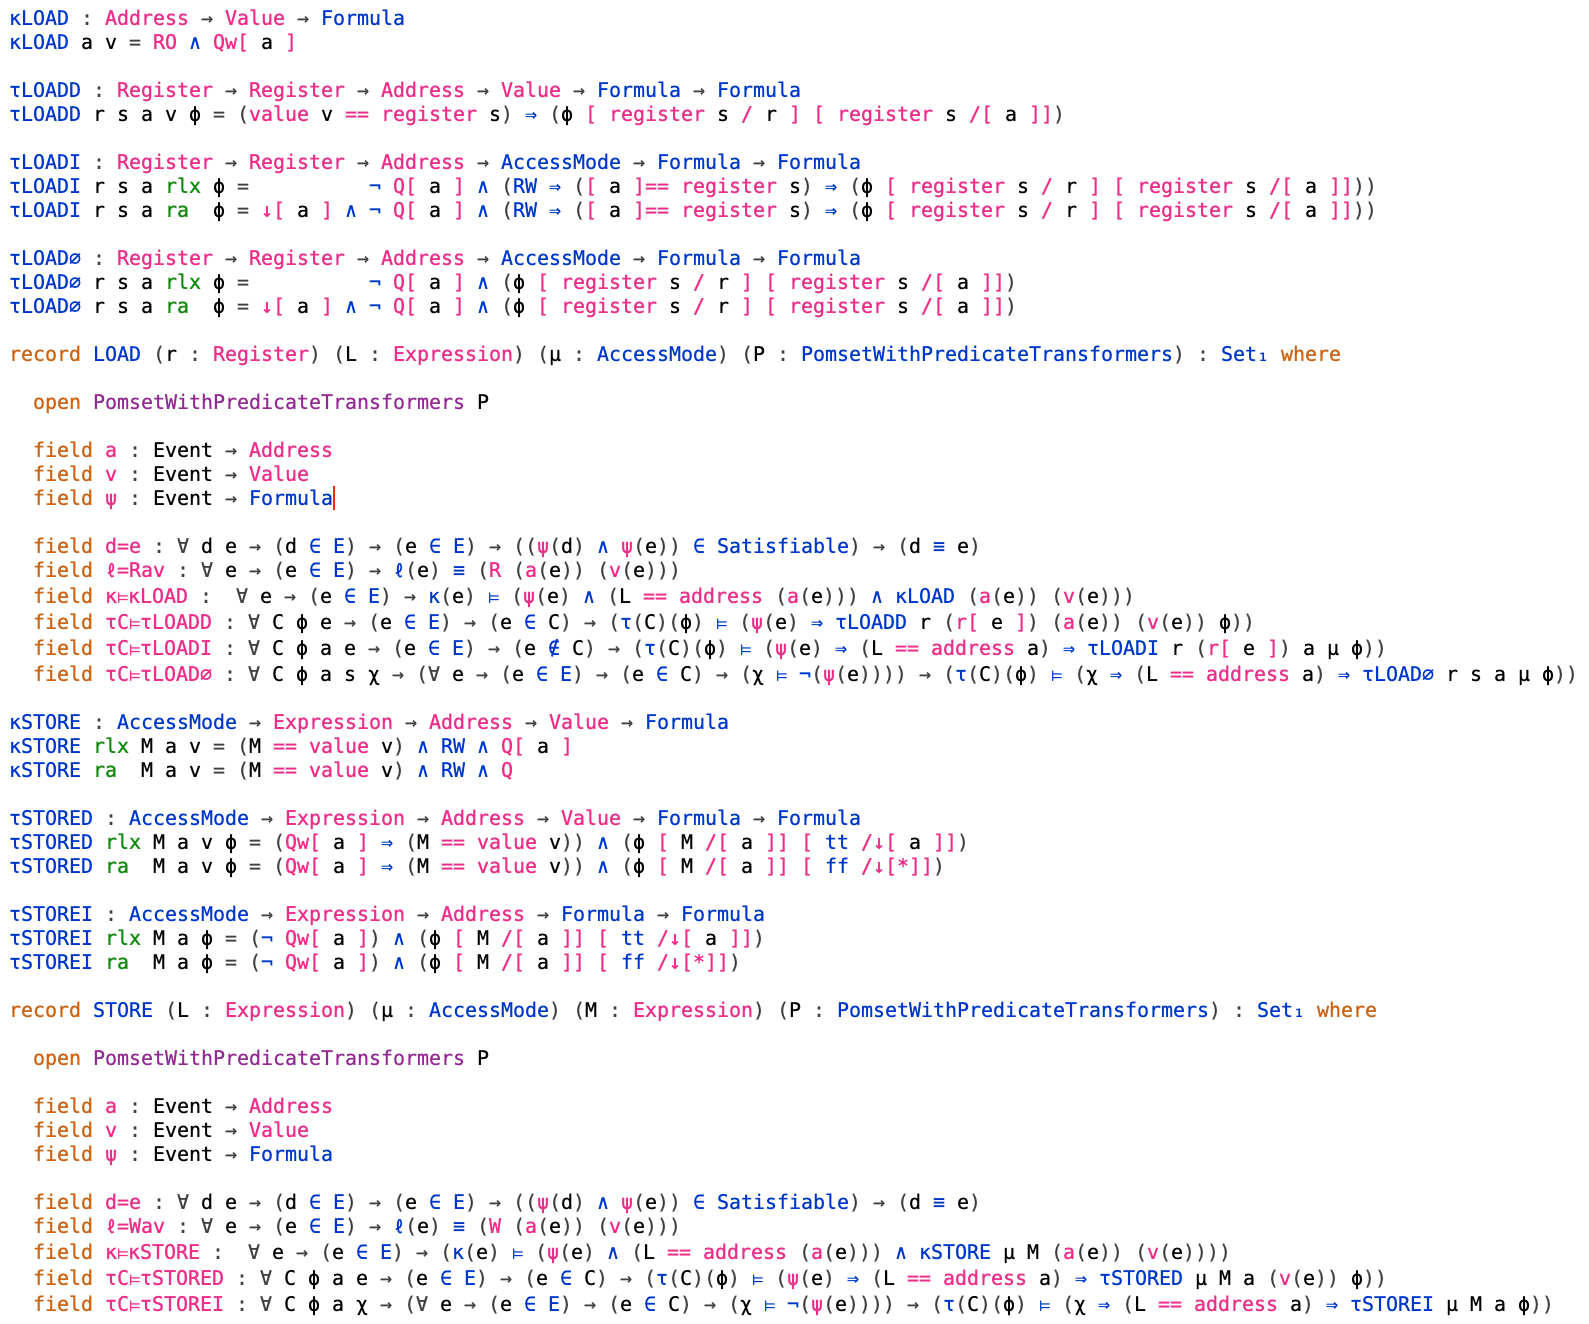
\includegraphics[width=\textwidth]{agda.png}
% \end{figure*}
